\documentclass{article}
\usepackage{../fasy-hw}
\usepackage{ wasysym }
\usepackage{graphicx}
%% UPDATE these variables:
\renewcommand{\hwnum}{1}
\title{Discrete Structures, Homework 1}
\author{Peyton Meeks (Peyton Meeks)}
\collab{n/a}
\date{due: 22 January 2021}

\begin{document}

\maketitle

This homework assignment should be
submitted as a single PDF file both to D2L and to Gradescope.

General homework expectations:
\begin{itemize}
    \item Homework should be typeset using LaTex.  (Note: if you are still
        having trouble with your setup, please reach out to the instructor and
        TA).
    \item Answers should be in complete sentences and proofread.
    \item You will not plagiarize.
    \item List collaborators at the start of each question using the
        \texttt{collab} command.
    \item Put your answers where the \texttt{todo} command currently is (and
        remove the \texttt{todo}, but not the word \texttt{Answer}).
\end{itemize}

% ============================================
% ============================================
\nextprob{Getting to Know Your Classmates}
\collab{n/a}
% ============================================
% ============================================

Find a different classmate for each of the following:
\begin{enumerate}
    \item Was born in the same month as you (year can be different).
        \paragraph{Answer} Discord handle: Patrick Schnable

    \item Has a shared hobby with you.
        \paragraph{Answer} Discord handle: Joey

    \item Has the same middle initial as you.
        \paragraph{Answer} Discord handle: Chandler

    \item Lives in a different building than you.
        \paragraph{Answer} Discord handle alec

    \item Has eaten at at least one restaurant or traveled to at least one city that you have not been
        (yet).
        \paragraph{Answer} Discord handle: emmaveld

\end{enumerate}

% ============================================
% ============================================
\nextprob{Why Proofs?}
\collab{n/a}
% ============================================
% ============================================

Much of this class is spent learning how to prove things.  Explain why it is
important to you, as a computer scientist, to know how to prove things
mathematically.

\paragraph{Answer}

Being able to prove things is the key to humanities' evolvement of understanding. Knowing how something works so that it can be duplicated and studied in a controlled setting is how we have developed the modern tools that we have today. 


% ============================================
% ============================================
\nextprob{A Proof}
\collab{n/a}
% ============================================
% ============================================

Prove that $6\Z \subset 2\Z$.

\paragraph{Answer}

Since the smallest element of 6Z is greater than the smallest element in 2Z but 6 and 2 are related by the fact that 2 is a factor of 6, that means all elements in 6Z are in 2Z but not all elements in 2Z are in 6Z.

% ============================================
% ============================================
\nextprob{Grace Hopper}
% ============================================
% ============================================

Write a short (1-2 paragraph) biography of Grace Hopper.
\textbf{In your own words}, describe who they are and why they are important in
the history of computer science.  If you use external resources, please provide
proper citations.

\paragraph{Answer}

Grace Hopper was one of what I consider first truly inovative computer scientists. She colaborated with a research team at Eckert-Mauchly Corporation to develop a program which would be the basis of all modern programming language. A linker converted the English language into code which a machine would understand. While doing all of this she served in the U.S. Naval Reserve as a rear admiral. Grace was selected to head a conference of computer scientists which, with her knowledge, led to the creation of the first independent computer programming language. This was one of the biggest revolutions of computer science in history. With an independent programming language, COBOL could be taught on a wide scale and understood by many. It did not require years of familiarization with multiple computer operating systems to be able to understand a program.

\footnote{"Grace Hopper." Wikipedia, Wikimedia Foundation, 22 Jan. 2021, \url{en.wikipedia.org/wiki/Grace_Hopper}.}

% ============================================
% ============================================
\nextprob{Bonus Question!}
\collab{n/a}
% ============================================
% ============================================

Use the `figure` environment to add a figure that provides the solution to
Exercises set 1.4, Problem 4.  Your figure can be hand drawn and scanned, or can
be made using a tool such as Inkscape.

	\begin{figure}[h]
		\caption{Solution to Exercises set 1.4 Problem 4}
		\centering
			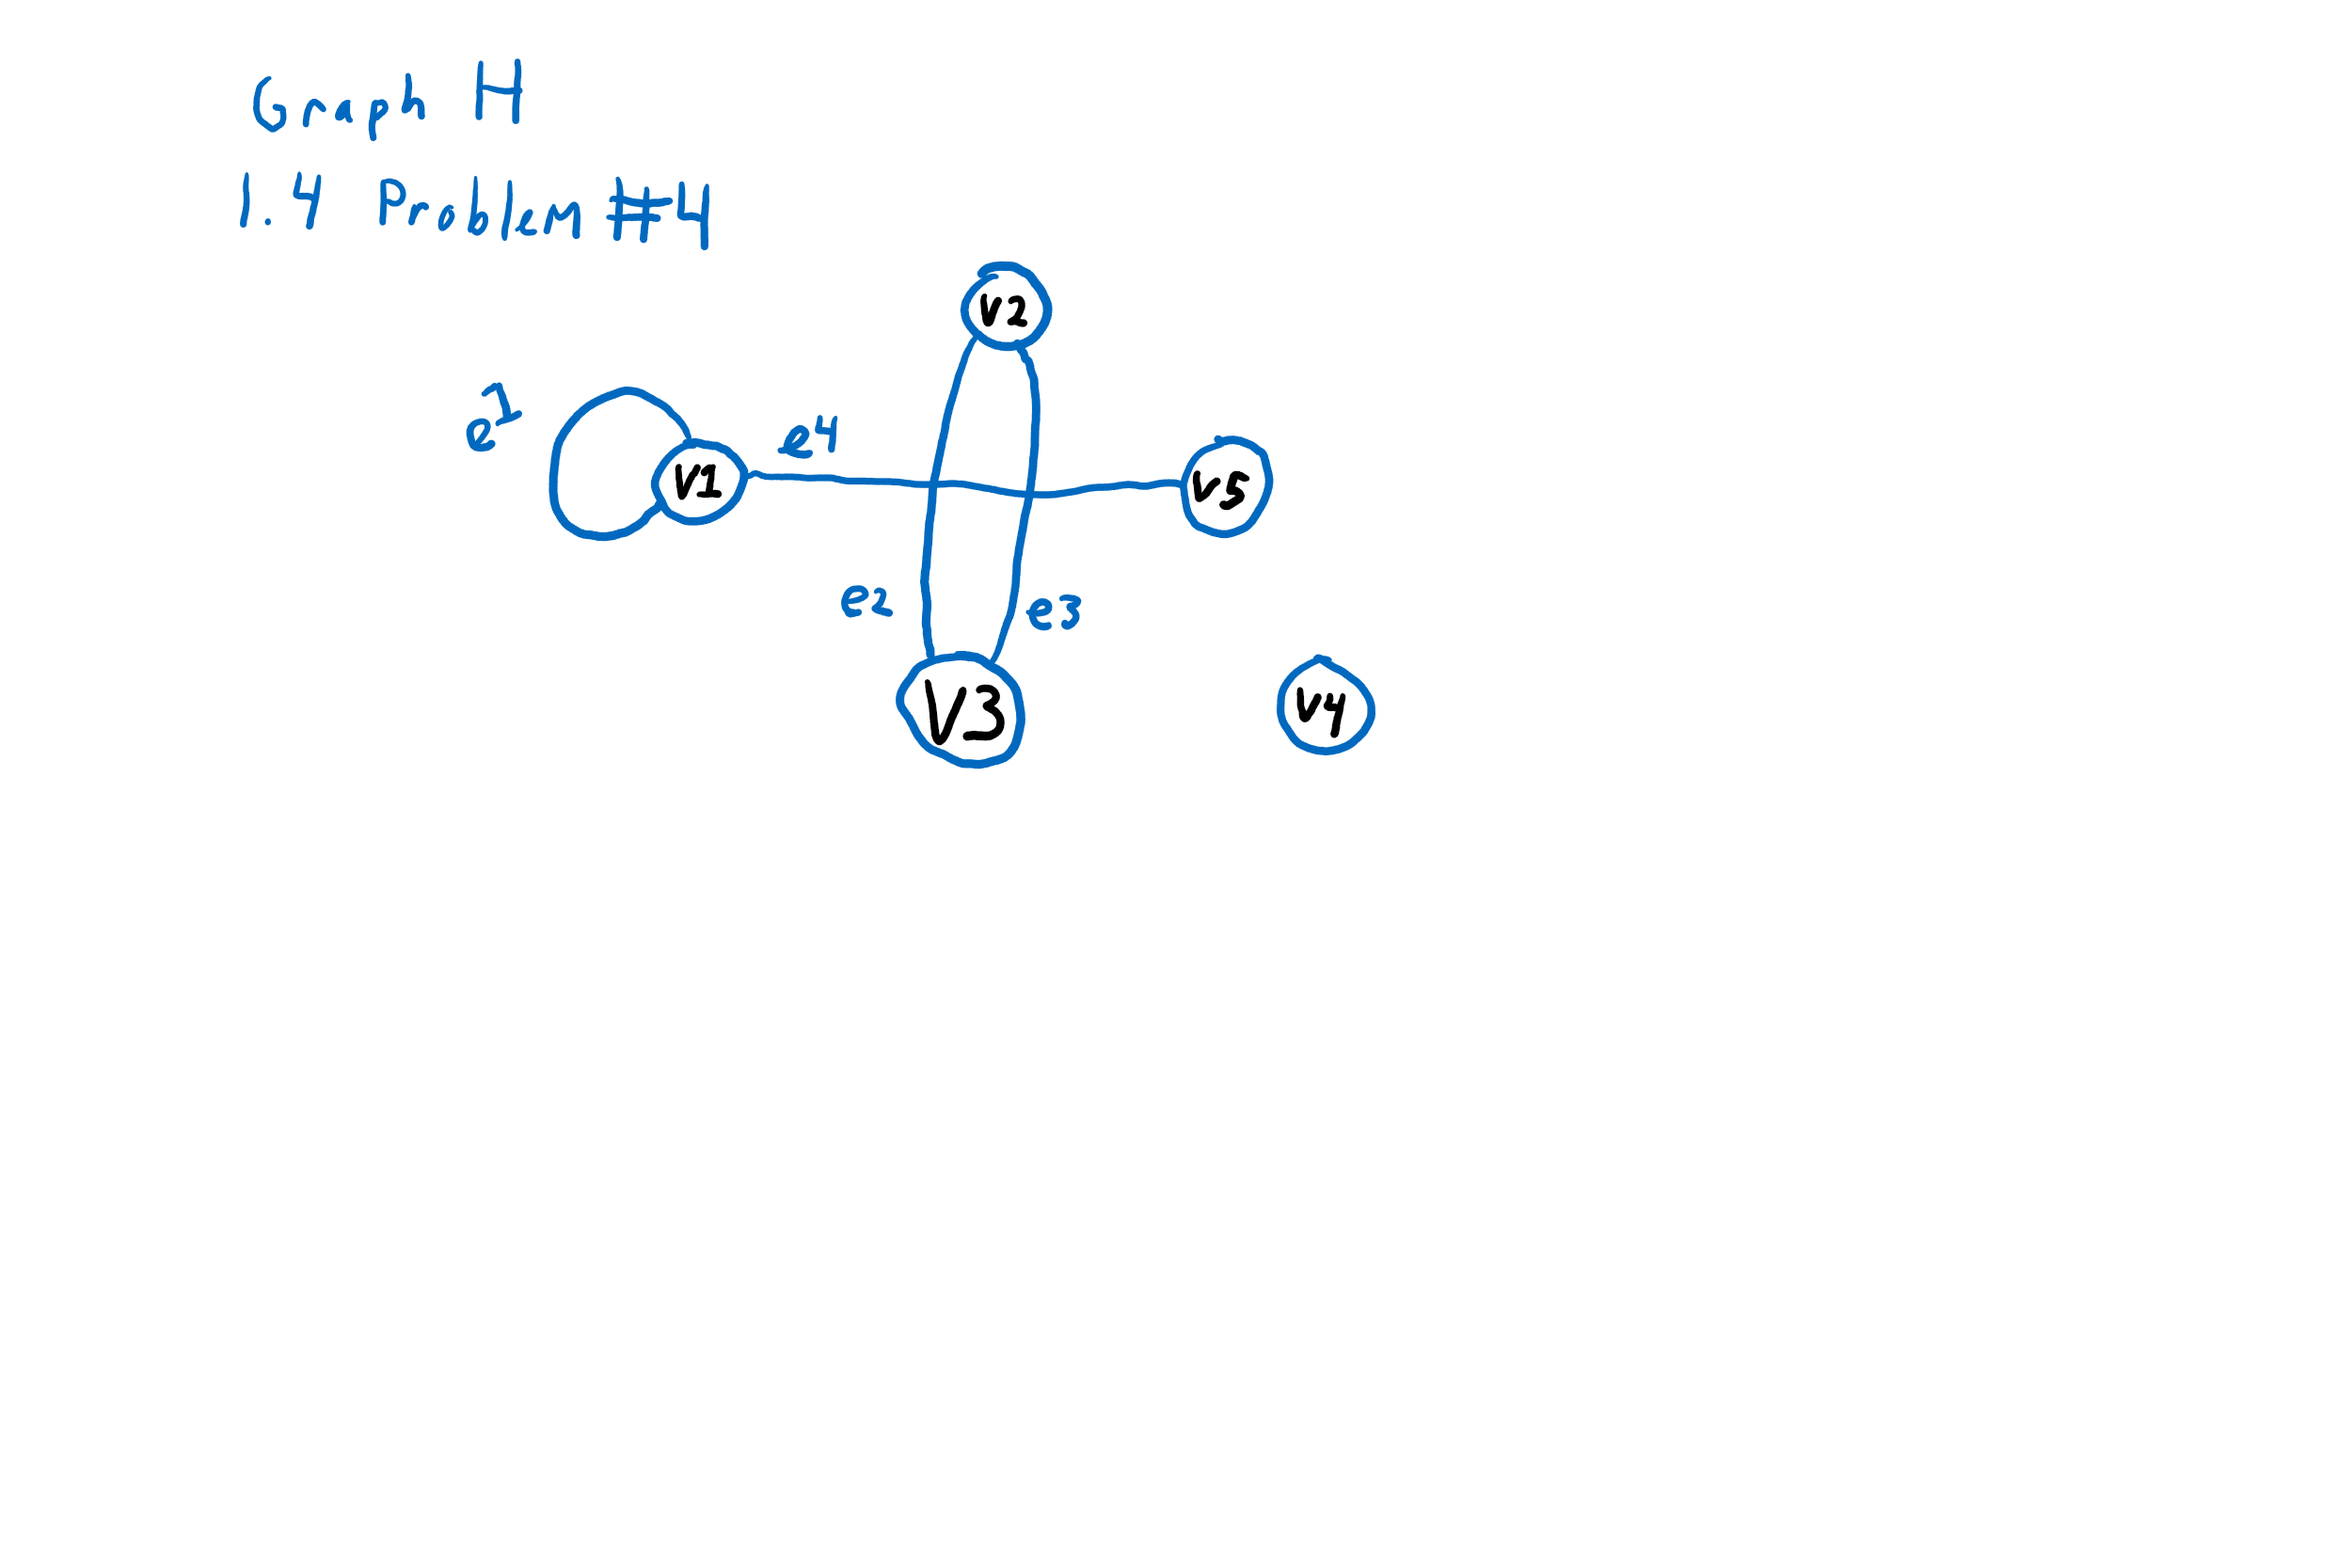
\includegraphics[width=0.5\textwidth]{H-1_Figure}
	\end{figure}

\end{document}

